\documentclass[11pt,a4paper]{article}
\usepackage[margin=2.2cm]{geometry}
\usepackage{amsmath,amssymb,booktabs,graphicx,xcolor}
\usepackage[colorlinks=true,citecolor=blue,urlcolor=blue]{hyperref}
\newcommand{\ttW}{t\bar t W}
\newcommand{\dd}{\mathrm{d}}
\newcommand{\Tr}{\operatorname{Tr}}
\newcommand{\as}{\alpha_s}
\newcommand{\GeV}{\,\mathrm{GeV}}
\title{Mixed production and decay corrections in trilepton $t\bar tW$ production}
\author{}
\date{Working draft: 14 September 2026}
\begin{document}
\maketitle
\begin{center}
\fbox{\parbox{0.9\linewidth}{\textbf{Status of this draft.}
The numerical campaign is in progress. The width results below have been
recomputed and checked. Fiducial cross sections, uncertainty bands and
phenomenological conclusions await validated integrations.}}
\end{center}
\begin{abstract}
Spin-correlated products of next-to-leading-order production and decay
densities contain mixed QCD corrections beyond their strict NLO expansion.
We formulate a study of these terms in direct trilepton $\ttW^\pm$
production, retaining separate renormalization scales for production, top
decay and antitop decay. Consistent total-width normalization makes the
inclusive branching cancellation a central validation test and isolates
the response to fiducial cuts. The comparison includes three treatments of
the W virtualities and five-flavour production with either massless or
massive-bottom decays. We specify observables, correlated scale and PDF
reductions, and the perturbative limitations of extra-jet distributions.
No phenomenological conclusion about the magnitude of the mixed terms is made
in this unfinished draft.
\end{abstract}

\section{Physics question and scope}

The question is whether the available mixed production--decay terms change
bottom-jet acceptance and charge-separated shapes, and whether any change
is stable under consistent width and scale choices. Differential measurements
by ATLAS and CMS motivate separating normalization and shape effects
\cite{ATLAS2024,CMS2026}; their particle-level definitions are not automatically
identical to the partonic selection below. The normalization of
unstable-particle decays requires particular care: changes of an integrated
decay width are not directly predictions for changes of a normalized
fiducial cross section \cite{Denner2012,Jezo2023}.
Full off-shell NLO calculations of trilepton $\ttW$ already provide
reference predictions \cite{Bevilacqua2020,Denner2020}. Our top
narrow-width approximation (NWA) has a different scope. A finite W width
inside independent production and decay blocks does not restore
single-resonant top contributions, alternative-history interference or
nonfactorizable exchanges between production and decay.

We retain the QCD-induced Born order $\as^2\alpha^6$ in the fully
leptonic final state and its NLO QCD stage corrections. The study excludes
subleading electroweak Born orders and NLO electroweak corrections, photon
initial states, showers, hadronization, multiple interactions and detector
effects. Products of available NLO factors do not establish NNLO precision.
In particular they contain neither the full second-order production
correction nor the full second-order correction within either top decay.

\section{Spin-correlated prescriptions and width expansion}

Let $P_0$ and $P_1$ denote the Born production density and its QCD
correction. For $i=t,\bar t$ let $D_{i,0}$ and $D_{i,1}$ be the
corresponding differential decay densities, normalized with the total
widths $\Gamma_{i,0}$ and $\Gamma_{i,0}+\Gamma_{i,1}$. Define
\begin{align}
B_{i,0}&=\frac{D_{i,0}}{\Gamma_{i,0}},&
B_{i,1}&=\frac{D_{i,1}}{\Gamma_{i,0}}
 -\frac{\Gamma_{i,1}}{\Gamma_{i,0}}B_{i,0}.
\end{align}
Spin contractions and the on-shell leptonic W-decay factors, when present,
are implicit. The strict NLO density is
\begin{align}
S=\Tr\big[(P_0+P_1)B_{t,0}B_{\bar t,0}
 +P_0B_{t,1}B_{\bar t,0}+P_0B_{t,0}B_{\bar t,1}\big].
\label{eq:strict}
\end{align}
The unexpanded product is
\begin{align}
\Pi=\Tr\left[(P_0+P_1)
\frac{D_{t,0}+D_{t,1}}{\Gamma_{t,0}+\Gamma_{t,1}}
\frac{D_{\bar t,0}+D_{\bar t,1}}{\Gamma_{\bar t,0}+\Gamma_{\bar t,1}}\right].
\label{eq:product}
\end{align}
These expressions refer to density contractions with combined phase spaces
and local subtraction counterevents. They are not products of histogram
$K$ factors. Equations~\eqref{eq:strict} and \eqref{eq:product} agree through
relative first order in $\as$.

The six comparisons are LO (Born production and decays), P (NLO production
and Born decays), D (Born production and the additive NLO decay terms),
S (strict NLO), $\Pi_D$ (the product with Born production), and $\Pi$.
All six use the same NLO PDFs and coupling. LO and P use LO top-width
denominators. The additive width counterterms are essential for
\begin{equation}
S=P+D-\mathrm{LO},
\end{equation}
which must hold for every infrared-safe bin and every common scale point.
The combinations $\Pi_D-D$ and $(\Pi-S)-(\Pi_D-D)$ distinguish effects
already present with Born production from effects involving $P_1$.
They are not homogeneous coefficients in $\as$.

To expose the formal second-order coefficient, collect numerator products
over the common LO width denominator as $A_0+A_1+A_2+A_3$, where the
index denotes relative QCD order, and write
$g_i=\Gamma_{i,1}/\Gamma_{i,0}$. Then
\begin{align}
\Pi&=\frac{A_0+A_1+A_2+A_3}{(1+g_t)(1+g_{\bar t})},\\
[\Pi-S]_2&=A_2-(g_t+g_{\bar t})A_1
 +(g_t^2+g_tg_{\bar t}+g_{\bar t}^2)A_0.
\end{align}
For a common decay scale the last expression becomes
$A_2-2gA_1+3g^2A_0$. Thus $A_2$ alone is not the complete second-order
term generated by the prescription. An eight-subset extraction must first
convert the selected denominators to the common LO convention; width-order
selection in the present implementation is species-wide.

For a fully integrated, consistently normalized on-shell decay the QCD
corrections cancel in its branching density. Consequently LO and D, and
separately P, S and $\Pi$, have the corresponding inclusive equalities
within Monte Carlo precision. This is a validation condition. A fiducial
selection breaks the cancellation through migration, so neither a small
inclusive change nor a narrower scale band determines the size of that
migration.

\section{Benchmark and independent W and bottom-mass treatments}

The baseline uses unpolarized proton beams at $\sqrt{s}=13$ TeV,
$m_t=172.5\GeV$, $M_W=80.385\GeV$ and $M_Z=91.1876\GeV$.
Masses and top Yukawa inputs are matched. The CKM matrix is diagonal.
The real $G_\mu$ input is $G_F=1.1663787\,10^{-5}\,\mathrm{GeV}^{-2}$
with
\begin{equation}
\alpha_{G_\mu}=\frac{\sqrt{2}G_F M_W^2}{\pi}
\left(1-\frac{M_W^2}{M_Z^2}\right),\qquad
\alpha_{G_\mu}^{-1}=132.233229791284.
\end{equation}
The model computes $M_W$ from these inputs. Both the dependent mass and
the generated numerical weak parameters must therefore be checked.

NNPDF40\_nlo\_as\_01180, member 0, LHAPDF ID 331700 and DataVersion 1
defines the nominal PDFs and the interpolated coupling \cite{NNPDF40}.
The same five-flavour coupling is used in production and decays. Replica
members 1--100 are retained for the PDF uncertainty. The metadata's fitted
bottom mass is not the on-shell mass used in a massive decay.

The W total width is held fixed in every comparison:
\begin{equation}
\Gamma_W^{\rm ref}=\Gamma_\ell
\left[3+6\left(1+\frac{\as^{\rm PDF}(M_W)}{\pi}\right)\right]
=2.097673562053\GeV,\qquad
\Gamma_\ell=\frac{G_FM_W^3}{6\pi\sqrt{2}}.
\end{equation}
This gives $B_e=B_\mu=0.108345431331$ for an on-shell W.
The top normalization widths are recomputed from the exact-mass NLO
coefficient and fixed-width convolution \cite{Campbell2012}.
The independent calculator's QCD coefficient
$C=\Delta\Gamma_{\rm QCD}^{\rm CLI}/\as^{\rm CLI}$ is matched to the PDF:
$\Gamma^{\rm NLO,PDF}=\Gamma_0+C\as^{\rm PDF}$.
The whole LO+NLO result is not rescaled.

\begin{table}[t]
\centering
\begin{tabular}{llrr}
\toprule
$m_b^{\rm decay}$ [GeV] & W in top width &
$\Gamma_{t,0}$ [GeV] & $\Gamma_t^{\rm NLO}$ [GeV]\\
\midrule
0 & on shell & 1.480628509250 & 1.353548521193\\
0 & fixed-width BW & 1.457601090044 & 1.332484829654\\
4.8 & on shell & 1.476533851481 & 1.351338725832\\
4.8 & fixed-width BW & 1.453538980794 & 1.330287530370\\
\bottomrule
\end{tabular}
\caption{Recomputed total top widths at $\mu_R=m_t$ using the fixed W
input and NNPDF4.0 coupling. The stored calculation retains full precision;
the displayed digits specify reproducibility, not physical accuracy.}
\label{tab:widths}
\end{table}

The \texttt{onshell} mode treats all three Ws as explicit on-shell decay
nodes. The \texttt{top-bw} mode uses full $t\to b\ell\nu$ currents but
retains an on-shell associated W. The \texttt{all-bw} mode additionally
uses the direct production current $pp\to t\bar t\ell\nu$. Tops remain
on shell in every mode. The internal W denominator is
$(q^2-M_W^2)^2+M_W^2(\Gamma_W^{\rm ref})^2$, with no associated-W mass
window. Only explicit W decay nodes receive a $1/\Gamma_W^{\rm ref}$
normalization: three, one, or zero such factors respectively. A direct
three-body current receives no extra branching factor. Both BW modes use
the same matched top-width row in Table~\ref{tab:widths}.

Production remains in the five-flavour scheme with massless bottom quarks
and bottom PDFs when the on-shell decay mass is changed from zero to
$4.8\GeV$. The massive decay amplitudes, virtual correction, phase space,
FKS mapping and total widths must all use that mass. This is a factorized
NWA approximation, not a four-flavour production calculation or a change
of PDF thresholds.

\section{Fiducial measurement and perturbative accuracy}

Each charge requires eight ordered flavour assignments for
$(W_t,W_{\bar t},W_{\rm assoc})\in\{e,\mu\}^3$. The initial
$(e,e,\mu)$ channel is a pilot, not the entire visible two-electron,
one-muon final state. Each ordered assignment is summed once, with no
manual factorial or universal multiplicity correction under cuts.

The same-sign leptons satisfy $p_T\geq20\GeV$ and the opposite-charge
lepton $p_T\geq10\GeV$. Electrons have $|\eta|<2.47$, excluding
$1.37<|\eta|<1.52$; muons have $|\eta|<2.5$.
Every opposite-sign same-flavour pair has $m_{\ell\ell}>12\GeV$ and lies
outside $|m_{\ell\ell}-91.1876\GeV|\leq10\GeV$. The analogous
trilepton Z window is vetoed. All final QCD partons are clustered with
anti-$k_T$, E-scheme recombination and $R=0.4$. Accepted jets have
$p_T\geq25\GeV$ and $|\eta|<2.5$. A jet containing a bottom or
antibottom is one ideal b jet, also when both are merged. Inclusive one-b
and nested two-b regions are measured.

Every selected lepton and accepted jet must obey
\begin{equation}
\Delta R(\ell,j)>\min\left(0.4,\,0.04+\frac{10\GeV}{p_{T,\ell}}\right).
\end{equation}
There is no missing-transverse-momentum cut. The radius alternatives
$R=0.3,0.5$ and the b thresholds 30 and 40 GeV are evaluated in the
same events. Light-jet thresholds remain at 25 GeV.
These are ATLAS-inspired theory selections \cite{ATLAS2024}.
The partonic overlap criterion and ideal b tags are not the experimental
object definitions; the calculation is not a direct data-fit template.

The principal shapes include subleading-b transverse momentum,
$m_{b\ell}^{\rm minimax}$, jet and lepton $H_T$, $S_T$ and same-sign
angular separations. The minimax uses both assignments of the two leading
b jets for each possible same-sign top lepton, and takes the smallest of
the four maximum pair masses. The Born endpoint
$m_{b\ell}^2=m_t^2-M_W^2$ motivates an endpoint study, but jet radiation
and pairing also populate tails.

\begin{table}[t]
\centering\small
\begin{tabular}{cll}
\toprule
Extra jets in two-b region & Strict NLO & Product\\
\midrule
0 & NLO, with veto-log limitations & Same NLO expansion plus selected terms\\
1 & LO for this multiplicity & Selected higher-order stage terms\\
2 & Zero & Mixed-stage double-real subset\\
3 & Zero & Production/top/antitop triple-real subset\\
\bottomrule
\end{tabular}
\caption{Accuracy for resolved non-bottom jets. The product does not
contain two emissions within the same stage. In particular, a second-extra-jet
distribution is only a subset of its complete leading coefficient.
No ratio to a vanishing strict-NLO prediction is defined.}
\label{tab:jets}
\end{table}

\section{Scale, PDF and statistical comparisons}

The primary production reference is
\begin{equation}
\mu^P_0=\frac12\left[m_{T,t}+m_{T,\bar t}+m_T(q_{\rm assoc})
+\sum_{j\in{\rm production\ radiation}}p_{T,j}\right],\qquad
m_T(q)=\sqrt{q_0^2-q_z^2}.
\end{equation}
For a direct associated current $q=p_\ell+p_\nu$, using its actual
virtuality; for an on-shell W its momentum is used. Decay scales are
independently centered on $m_t$. The four variation factors
$(\xi_R^P,\xi_F^P,\xi_R^t,\xi_R^{\bar t})\in\{1/2,1,2\}^4$
produce 81 weights. Excluding only the two antipodal production corners
leaves the main 63-point envelope. The shared-decay comparison has 21
points and the fully common scale only three. There is no additional
restriction on the ratio of the decay scales.

At each identical scale point we form $\Pi-S$, $\Pi/S$, each normalized
shape and acceptance, the two-b-given-one-b efficiency and the zero-extra-jet
fraction. Only then are envelopes taken. Charge ratios and
$A_W=(\sigma_+-\sigma_-)/(\sigma_++\sigma_-)$ use matched points in both
charges. The observable $A_W$ is the associated-W charge asymmetry.
Decay and production bands are not combined as Gaussian errors.
Native lepton-resolved production $H_T/2$ in \texttt{all-bw} and the
fixed scale $m_t+M_W/2=212.6925\GeV$ are separate central prescriptions.

For a decay-scale factor $\xi$, the matched width follows
\begin{equation}
\Gamma_t^{\rm NLO}(\xi m_t)=\Gamma_{t,0}+
[\Gamma_t^{\rm NLO}(m_t)-\Gamma_{t,0}]
\frac{\as^{\rm PDF}(\xi m_t)}{\as^{\rm PDF}(m_t)}.
\end{equation}
The top and antitop evaluate this function independently. The W input
does not vary. Direct reruns at asymmetric scales must validate the
reweighted result and the local subtraction-scale cancellation.

PDF-derived observables are constructed member by member, preserving
flavour and charge correlations, before the one-standard-deviation
replica reduction. Member 0 remains nominal; any difference from the
replica mean is recorded for nonlinear observables. PDF-family and
strong-coupling comparisons require newly matched top NLO widths.

The calculation uses the fNLO branch of MadGraph5\_aMC@NLO
\cite{MG5} with FKS subtraction \cite{FKS}, FastJet \cite{FastJet}
and LHAPDF6 \cite{LHAPDF6}. The exact checkout and dependency versions
are recorded with the inputs.

Monte Carlo errors on ratios and normalized shapes require covariance.
The stored histogram errors alone do not provide all bin/rate or
cross-run covariance. We preserve the joint vectors from equal-count
integration batches, conditional on their trained importance grids.
For subprocess/channel stratum $s$ with $N_s$ batches $X_{sj}$ before
their $1/N_s$ weights, the estimator is $\sum_s\overline X_s$ and its
conditional covariance is
\begin{equation}
 \widehat C=\sum_s\frac{1}{N_s(N_s-1)}
 \sum_{j=1}^{N_s}(X_{sj}-\overline X_s)(X_{sj}-\overline X_s)^T.
\end{equation}
For nonlinear observables we delete a complete batch from one stratum
at a time and add the independent stratum variances. This preserves
bin/normalization and scale/PDF correlations, but does not guarantee
coverage for poorly sampled tails or adaptive stopping. New worker streams
include the refinement stage, with actual initialization pairs audited across
training and every refinement. Independent full-run convergence
checks remain necessary; identical seeds in different samplers do not
establish correlation. Repeated estimates of one process must be combined
statistically, whereas disjoint charge/flavour channels are summed.
The main campaign is prepared with five complete independent integrations
per flavour, charge and prescription, each with fresh importance-grid
training. For these ensembles, the uncertainty estimator uses the scatter
between complete runs. Let $g$ label an independent ensemble and
$\theta_{g(-j)}$ a vector of observables evaluated after deleting run $j$
from ensemble $g$, with every other ensemble held at its mean. Then
\begin{equation}
 \widehat C_{\rm runs}=\sum_g\frac{R_g-1}{R_g}
 \sum_{j=1}^{R_g}
 (\theta_{g(-j)}-\overline\theta_g)
 (\theta_{g(-j)}-\overline\theta_g)^T,
 \qquad
 \overline\theta_g=\frac{1}{R_g}\sum_j\theta_{g(-j)}.
\end{equation}
The reported central prediction is the observable of the ensemble means.
Flavours are summed within each charge; a combined charge shape is
normalized only after adding the two raw spectra and their parent rates.
Conditional batch variances are retained as diagnostics and are not added
again to this between-run covariance. A physical state reused in several
W-treatment, bottom-mass or parameter comparisons enters once, preserving
their shared statistical uncertainty. In particular, the intermediate
top-BW prediction enters the top-W and associated-W differences with
opposite signs. Independent charges, prescriptions and flavours are not paired
by run index. For charge-asymmetry sensitivity we retain absolute changes,
which remain defined when the asymmetry crosses zero. This procedure
preserves the measured correlations; five runs alone do not establish
coverage in poorly sampled bins or under adaptive stopping.
The target precision is initially below one percent for fiducial rates
and one to two percent in retained populated shape bins. A claimed shift
must have an MC error below approximately one third of its magnitude.

\section{Validation and numerical results}
The matched width calculations in Table~\ref{tab:widths}, the five
specified PDF coupling checkpoints and all nine signed top/antitop width
and counterterm combinations pass their runtime checks. All 101 members
of the prescribed NNPDF4.0 set are installed and hashed. The measurement
regressions use the actual FastJet wrapper. Generator validation includes
pole cancellation, soft/collinear subtraction checks, analytic/MadLoop
decay-virtual comparisons and exclusive-jet partition identities.
Analytic-provider validation requests MadLoop precision of $10^{-10}$
or better before the independent $10^{-8}$ density comparison.
Numerical fixes to sparse-bin accumulation, near-endpoint phase space,
refinement seeding and massive Born-map ordering are regression-tested;
failed or affected legacy attempts retain their original provenance and
are excluded from certified comparisons.

All six on-shell prescriptions have completed initial single-assignment
pilots for both charges. The independent $S-P-D+\mathrm{LO}$ checks have
maximum absolute central-bin residuals 2.986 and 2.976 MC errors for W$^+$
and W$^-$, over 2802 and 2806 nonzero-error bins. These correlated residuals
are not a global goodness-of-fit test or a publication-precision check.
Earlier stable-production branching tests are provisional because a
subsequent audit found repeated refinement streams in the two-round W$^+$
reference. Fresh NLO inclusive normalization remains required.

The independent native associated-current versus factorized-decay LO
comparison at matched fixed scales gives a decayed/expected ratio
$0.9931\pm0.0041$. The maximum absolute scale/PDF conditional residuals
are 1.71/1.79 MC errors. The native result is multiplied by the two
matched top branching densities only; the associated current receives
no extra branching factor. Actual sampling counts and distinct stage
streams are audited. This supports fixed-scale LO normalization, while
the convergence discrepancy between finite linear/current-proposal
samples still precludes an efficiency or full-support convergence claim.

The latest fixed-source W$^+$ S/$\Pi$ controls use the corrected stage
seeding and Born mapping. All four pass the complete histogram, weight,
virtual and batch audits. Their conditional fiducial ratios appear in
Table~\ref{tab:freshpilots}; none resolves a product shift at the specified
precision. Maximum absolute paired inclusive decay-scale residuals are
0.95/1.13 MC errors for all-BW S/$\Pi$ and 0.27/1.25 for on-shell S/$\Pi$.
These paired cancellations do not replace the independent absolute NLO
current normalization or tests of retraining and sparse-tail convergence.

Direct asymmetric decay scales, $\mu_R^t=2m_t$ and
$\mu_R^{\bar t}=m_t/2$, have now been compared with the corresponding
reweighted coordinates in independent on-shell W$^+$ samples. The direct
one-/two-b rate ratios to reweighting are
$0.9621\pm0.0429$ / $1.0120\pm0.0401$ for S and
$0.9993\pm0.0199$ / $0.9996\pm0.0250$ for $\Pi$.
The 36 distinct matching physical scale points give maximum absolute
rate residuals of 1.30 and 1.57 conditional MC errors. Across the six
normalized spectra and their matching scale coordinates, the maximum is
3.03 MC errors; the few entries above three are correlated bin/scale
comparisons, not a global significance. Each new sample passes 768
analytic-virtual comparisons, and its 130 actual stage initializations
are disjoint from the reference and other controls. These results support
asymmetric reweighting at the measured precision; QES cancellation,
direct BW production-scale checks and the central-scale diagnostics remain
in progress.

\paragraph{Matched literature configuration.}
The first W$^+$ LO/P/S reference calculation uses the separate inputs,
selection and fixed scale of Ref.~\cite{Bevilacqua2020}, including NNPDF3.0
and constant total top widths under scale variation. Under that reference's
unexpanded-width convention, the additive numerator reconstructed as
$[S+2g\,\mathrm{LO}]/(1+g)^2$, $g=\Gamma_{t,1}/\Gamma_{t,0}$, gives
$122.9\pm2.9$ ab, compared with the published rounded 123.0 ab.
The higher-statistics production-only prediction is $126.52\pm0.39$ ab
versus 127.0 ab. These conditional joint-batch errors use 410 distinct stage initializations
across the three independently sampled prescriptions. The reconstructed
NWA seven-point envelope is $[114.2,129.4]$ ab, compared with the published
rounded $[114.3,129.3]$ ab.
The P residual is $-1.21$ times our joint MC error; the reference tables
supply no MC errors, so this is not a combined statistical pull.
An independent lower-statistics P run differs by $2.08\pm1.05$ ab;
the largest absolute difference across the common-scale grid is 2.05
conditional MC errors. Both estimates are retained as convergence evidence.
The NWA reconstruction retains the previously audited LO and S samples;
it is not an additional independent strict-NLO calculation.
The completed W$^-$ calculation gives reconstructed NWA
$67.90\pm0.69$ ab versus 68.0 ab and production-only $70.85\pm0.96$ ab
versus 69.8 ab. These conditional joint errors use 282 distinct stage
initializations, with no overlap between prescriptions.
All raw common-scale weights, workers and stage histories are retained.
These matched references do not release the full phenomenological
campaign by themselves.

The inclusive dilepton-$t\bar t$ calibration uses separate NNPDF3.1 NLO
inputs and common fixed numerator scales $\mu=m_t$, with the supplied
total-width coefficients held fixed under variation~\cite{Behring2019}.
The comparison uses the authors' June 2019 normalized-distribution update.
Against the supplied ten-bin $\Delta\phi(\ell^+,\ell^-)/\pi$ curves, the
largest central-bin residuals are 1.65 combined MC errors for
$S({\rm bin})/S({\rm total})$ and 1.60 for its NLO-expanded normalization.
The latter expansion concerns the normalized observable, independently
of the expansion of the top-width denominators.
Our conditional bin errors range from 1.9--5.9\% and 2.8--9.1\%, respectively;
the supplied central-bin MC errors enter in quadrature. Reference
inter-bin covariance is unavailable, so these correlated residuals are
not a global goodness-of-fit test. All 513 LO/S/$\Pi$ training/refinement
initializations are distinct. This establishes pilot-level compatibility;
percent-level shape precision and retraining coverage remain unverified.
Direct scale/QES and absolute-normalization checks are in progress.

\begin{table}[ht]
\centering
\begin{tabular}{llcc}
\toprule
W treatment & Decay $m_b$ & $\Pi/S$, one-b & $\Pi/S$, two-b\\
\midrule
On shell & $0$ & $0.982\pm0.043$ & $0.993\pm0.037$\\
On shell & $4.8\GeV$ & $1.019\pm0.028$ & $1.000\pm0.032$\\
All BW & $0$ & $1.025\pm0.039$ & $0.939\pm0.043$\\
All BW & $4.8\GeV$ & $0.944\pm0.040$ & $0.895\pm0.049$\\
\bottomrule
\end{tabular}
\caption{Fixed-source technical W+ $e,e,\mu$ pilots after the Born-order fix,
not full direct-flavour predictions.
Errors are conditional independent-stratum batch estimates, including
correlations of weights; they are not scale or PDF uncertainties.}
\label{tab:freshpilots}
\end{table}

\paragraph{W-treatment companions.}
The six massless S/$\Pi$ samples per charge provide matched comparisons
of all three W treatments, using the common dynamic W-system scale and
the appropriate top widths. All 1624 actual training/refinement
initializations are distinct across these twelve samples. The conditional
double ratio $(\Pi/S)_{\rm all\mbox{-}BW}/(\Pi/S)_{\rm on\ shell}$ is
$1.044\pm0.060$ ($0.946\pm0.056$) for W$^+$ in the one-b (two-b)
selection and $1.139\pm0.097$ ($1.089\pm0.079$) for W$^-$.
Figure~\ref{fig:wtreatmentpilot} also separates the top-W and associated-W
changes. These pilots do not resolve a W-treatment change of the product
ratio. Their three comparisons share samples: the top-BW contribution
enters the two adjacent changes with opposite signs. The stored joint
covariance reproduces the additive closure of the changes in $\Pi-S$
and $\Pi/S$; treating the three errors as independent would lose this
relation. All 81 scale points and 101 PDF members are retained.
For the five selected normalized spectra (lepton $H_T$, leading- and
subleading-b $p_T$, $m_{b\ell}^{\rm minimax}$ and leading-lepton $p_T$),
the largest absolute nominal-bin change in $\Pi/S$ is 2.76 conditional
MC errors among bins with finite, nonzero errors. This is not a global
significance test or a bound on unsampled tails. Full-flavour sums and
independent-retraining convergence remain required.

\begin{figure}[t]
\centering
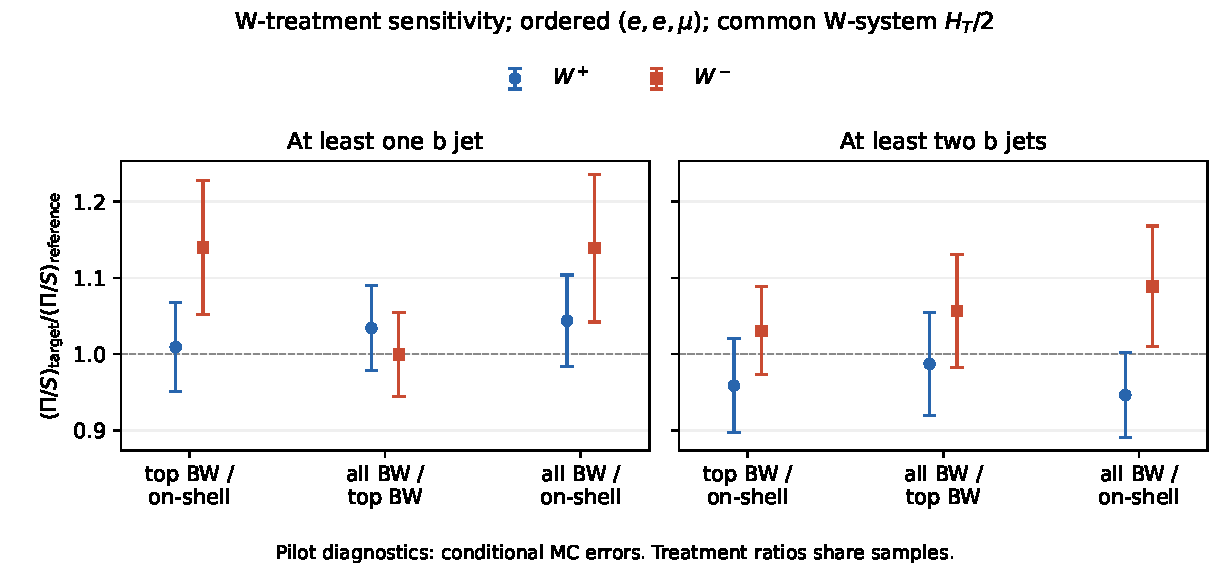
\includegraphics[width=\linewidth]{../figures/w_treatment_pilot_width_mass_v2.pdf}
\caption{W-treatment changes of the product/strict ratio for the single
ordered $e,e,\mu$ assignment in both charges. Bars are conditional MC
errors, and the three treatment ratios share samples. These pilot
diagnostics use matched widths and common dynamic production scales;
they are not full-flavour predictions or a convergence certification.}
\label{fig:wtreatmentpilot}
\end{figure}

The massive-decay companions retain massless five-flavour production:
88 source files for production, flavour data and virtuals, and the production-owned FKS
records match the massless export exactly. The massive parameter-card
round trip and all 120 pre-integration pole checks pass. The first massive
strict-sum pilot completed, but its product companion stopped on a local
Born-snapshot alignment check. The cause was a different daughter ordering
in the canonical tree and the massive NLO context. An explicit-identity
permutation fix passes 2400 deterministic Born-map checks, and fresh
on-shell and all-BW massive S/Pi pairs pass the full pilot audits.
The massive/massless double ratio of $\Pi/S$, formed before scale/PDF
reduction with four independent sample/stratum ensembles, is
$1.038\pm0.053$ ($1.007\pm0.050$) in the on-shell one-b (two-b) selection
and $0.921\pm0.053$ ($0.953\pm0.067$) for all BW. These conditional MC
errors do not resolve a mass dependence at the specified precision.
The completed W$^-$ companions give double ratios
$1.146\pm0.090$ ($1.109\pm0.064$) for the on-shell one-b (two-b)
selection and $0.976\pm0.059$ ($0.955\pm0.070$) for all BW.
These single-assignment results also do not resolve a mass dependence.
Independent-retraining convergence, small-mass continuity and the main
flavour-summed mass/width-scheme comparison remain open.

\paragraph{Generated narrow-W limit.}
The 21 massless-decay LO/S/$\Pi$ tests now contain an on-shell reference
and top-BW/all-BW samples at
$\epsilon=\Gamma_W/\Gamma_W^{\rm ref}=1,0.2,0.05$ for each prescription.
All use the common fixed scale $m_t+M_W/2=212.6925\GeV$ for production,
both decay numerators and the reference coupling in the top widths.
Weak couplings remain fixed while the matched top widths are recalculated.
The finite comparison is $\epsilon^3\sigma_{\rm BW}/\sigma_{\rm on\ shell}$:
each selected leptonic W density supplies one inverse power of $\epsilon$.
This factor is applied once to the reported cross sections, with no change
to the generated event weights and no additional branching factors.

At $\epsilon=0.05$, the LO two-b ratios are
$1.0028\pm0.0067$ (top BW) and $1.0032\pm0.0063$ (all BW).
For $\Pi$ they are $1.023\pm0.038$ and $1.022\pm0.040$;
for S they are $0.847\pm0.121$ and $0.872\pm0.124$.
These are conditional joint MC errors from independent run/beam strata,
with the common on-shell reference propagated to all width points.
The S comparison is limited particularly by the imprecise on-shell
fiducial reference. It does not establish percent-level NLO continuity.
Across six coarsened spectra at the narrowest width, the largest absolute
normalized-bin residuals are 2.13, 2.74 and 2.05 conditional MC errors
for LO, S and $\Pi$, respectively. These correlated bin residuals are
diagnostics, not a global goodness-of-fit test. The coarse bins retain
the original range and are summed before normalization to the matching
fiducial rate. Unmeasured continuous overflows are not folded into them.
All 81 scale and 101 PDF coordinates are retained in the comparison arrays.

\begin{figure}[ht]
\centering
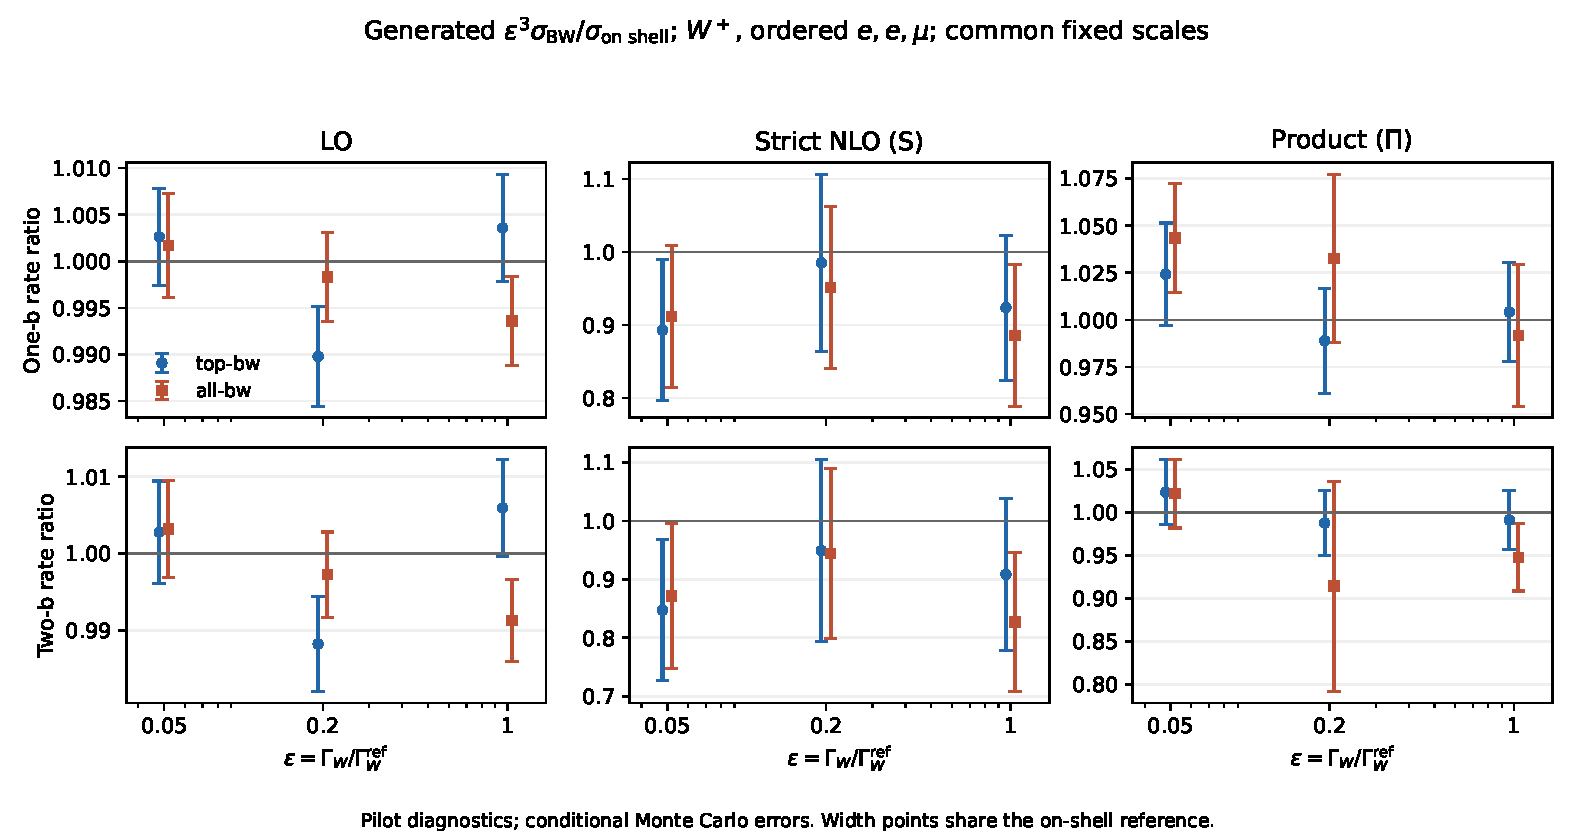
\includegraphics[width=\linewidth]{../figures/generated_narrow_w.pdf}
\caption{Generated narrow-W diagnostics for the single ordered W+
$e,e,\mu$ assignment at common fixed scales. Vertical bars show conditional
MC errors; points at different widths share the on-shell reference.
Horizontal offsets separate the two W treatments. Each panel has its own
vertical scale. These pilot results are not full-flavour predictions or a
percent-level NLO convergence certification.}
\label{fig:narrowW}
\end{figure}

Full-flavour and NLO varied-weight normalization, direct scale
reweighting checks, small-mass validation and integration convergence
remain open. Matched ttW and dilepton-ttbar reference pilots have completed;
their subsequent direct-scale and absolute-normalization tests are in progress.


\section{Interpretation and remaining limitations}

Any conclusion must distinguish a mixed-stage correction, a W-treatment
change, a production-scale-definition change and a decay-bottom-mass
effect. A narrower product envelope, if observed, measures the response
of this particular prescription. It cannot compensate for missing
same-stage terms. Extra-jet observables have the limitations in
Table~\ref{tab:jets}, and small veto scales can introduce large logarithms.
Recent NNLO ttW production results include an explicit two-loop amplitude
in the generalized leading-colour approximation \cite{Becchetti2026}.
That advance does not supply the complete spin-correlated second-order
production-and-decay density needed here.
The matched dilepton $t\bar t$ calculation is a calibration; compatibility
with complete NNLO production-and-decay information \cite{Czakon2020}
must be established before a coefficient-level comparison.
Public histograms exist, but their PDF order, cuts, differential decay scales
and fixed inclusive-width convention differ from this benchmark. They do not
directly isolate the missing same-stage coefficient.
The final conclusions will be written after the numerical validation,
full flavour sum and robustness campaign.

\begin{thebibliography}{99}
\raggedright
\bibitem{MG5}
J.~Alwall et al.,
\emph{The automated computation of tree-level and next-to-leading order
differential cross sections, and their matching to parton shower simulations},
\href{https://arxiv.org/abs/1405.0301}{arXiv:1405.0301}.
\bibitem{FKS}
S.~Frixione, Z.~Kunszt and A.~Signer,
\emph{Three-jet cross sections to next-to-leading order},
\href{https://arxiv.org/abs/hep-ph/9512328}{arXiv:hep-ph/9512328}.
\bibitem{FastJet}
M.~Cacciari, G.~P.~Salam and G.~Soyez,
\emph{FastJet user manual},
\href{https://arxiv.org/abs/1111.6097}{arXiv:1111.6097}.
\bibitem{LHAPDF6}
A.~Buckley et al.,
\emph{LHAPDF6: parton density access in the LHC precision era},
\href{https://arxiv.org/abs/1412.7420}{arXiv:1412.7420}.
\bibitem{Campbell2012}
J.~M.~Campbell and R.~K.~Ellis,
\emph{Top-quark processes at NLO in production and decay},
\href{https://arxiv.org/abs/1204.1513}{arXiv:1204.1513}.
\bibitem{Denner2012}
A.~Denner, S.~Dittmaier, S.~Kallweit and S.~Pozzorini,
\emph{NLO QCD corrections to off-shell top-antitop production with leptonic
decays at hadron colliders},
\href{https://arxiv.org/abs/1207.5018}{arXiv:1207.5018}.
\bibitem{Jezo2023}
T.~Je\v{z}o, J.~M.~Lindert and S.~Pozzorini,
\emph{Resonance-aware NLOPS matching for off-shell $t\bar t+tW$
production with semileptonic decays},
\href{https://arxiv.org/abs/2307.15653}{arXiv:2307.15653}.
\bibitem{Bevilacqua2020}
G.~Bevilacqua, H.-Y.~Bi, H.~B.~Hartanto, M.~Kraus and M.~Worek,
\emph{The simplest of them all: $t\bar tW^\pm$ at NLO accuracy in QCD},
\href{https://arxiv.org/abs/2005.09427}{arXiv:2005.09427}.
\bibitem{Denner2020}
A.~Denner and G.~Pelliccioli,
\emph{NLO QCD corrections to off-shell $t\bar tW^+$ production at the LHC},
\href{https://arxiv.org/abs/2007.12089}{arXiv:2007.12089}.
\bibitem{NNPDF40}
R.~D.~Ball et al.,
\emph{The path to proton structure at one-percent accuracy},
\href{https://arxiv.org/abs/2109.02653}{arXiv:2109.02653}.
\bibitem{ATLAS2024}
ATLAS Collaboration,
\emph{Measurement of the total and differential cross-sections of
$t\bar tW$ production in $pp$ collisions at $\sqrt{s}=13$ TeV with the
ATLAS detector},
\href{https://arxiv.org/abs/2401.05299}{arXiv:2401.05299}.
\bibitem{CMS2026}
CMS Collaboration,
\emph{Measurements of ttW differential cross sections and the leptonic charge
asymmetry at $\sqrt{s}=13$ TeV}, JHEP 03 (2026) 083,
\href{https://arxiv.org/abs/2509.13512}{arXiv:2509.13512}.
\bibitem{Becchetti2026}
M.~Becchetti et al.,
\emph{NNLO QCD predictions for $t\bar tW$ production at hadron colliders},
\href{https://arxiv.org/abs/2606.09503}{arXiv:2606.09503}.
\bibitem{Behring2019}
A.~Behring, M.~Czakon, A.~Mitov, A.~S.~Papanastasiou and R.~Poncelet,
\emph{Higher order corrections to spin correlations in top quark pair
production at the LHC}, Phys.\ Rev.\ Lett.\ 123 (2019) 082001,
\href{https://arxiv.org/abs/1901.05407}{arXiv:1901.05407}.
The June 2019 normalized-distribution update is available on the
\href{https://www.precision.hep.phy.cam.ac.uk/results/ttbar-decay/}{authors' data page}.
\bibitem{Czakon2020}
M.~Czakon, A.~Mitov and R.~Poncelet,
\emph{NNLO QCD corrections to leptonic observables in top-quark pair
production and decay},
\href{https://arxiv.org/abs/2008.11133}{arXiv:2008.11133}.
\end{thebibliography}
\end{document}
